\section{Proposal}

With Swift, the available access control mechanism is  ACL ( access Control List) which specify who can or cannot access an object or a file. In this approach, if someone can access a document, he/she gets the full content of the document which is an all or nothing approach.  Figure \ref{fig:swiftfile} and \ref{fig:zwiftfile}  illustrates the situation where in the former case, a file is accessed in all / nothing approach and in the later case the file can be selectively accessed by different users. But we believe that   zerovm enables more sophisticated cases which require more flexible access control than the ACL. For example,  a hospital that stores patient medical record in the cloud,  wants all its doctor, nurse or patient access the partial content based on the available role of the requester.  So, along with the content, the owner (in this case, the hospital) of an object/file may need to specify who can access how much of the content.

\begin{figure}[h!] 
  \centering
    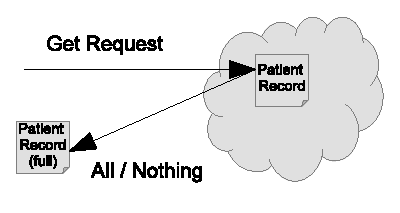
\includegraphics[width=0.3\textwidth]{eps/swift_file}
 \caption{A picture of a gull.}
\label{fig:swiftfile}
\end{figure}

\begin{figure}[h!]
  \centering
    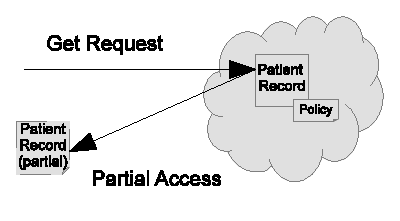
\includegraphics[width=0.3\textwidth]{eps/zwift_file}
 \caption{A picture of a gull.}
\label {fig:zwiftfile} 
\end{figure}




listing \ref{patient Record}, shows a sample file to be stored in the object store. For our example, we specify three different user roles namely, doctors, patient, and nurse.
A sample policy to be specified by the content owner is shown below.


\begin{listing}
\begin{minted}[frame=single,
               framesep=3mm,
               linenos=true,
               xleftmargin=21pt,
               tabsize=2]{js}
{
 "medical_record": {
 "Personal_information": {
	    "Name": "Monica Latte",              
           "Gender": "Female",
           "Contact By": "Phone"
       },
       "identification": {
         "Soc_Sec_No": "444-444",
         "Patient_ID": "0000-44"
       },
      "physical_exam": {
	  "appearance": "well developed",
	  "eyes": "conjunctiva"
	},
       "Medications": [
            "PRINIVIL TABS 20 MG ",
            "Last Refill: #30 x 2 "
        ]    
      
    }
}

\end{minted}
\caption{ Content of file patient\_record.json stored in the Object Storage} 
\label{patient Record}
\end{listing}

\begin{enumerate}

  \item  personal information as specified by jsonpath //personal\_information (shown in line 2 to 7), should be labeled 'personal' and only the owner of the file should be able access objects labeled personal .

  \item Identification information as specified by jsonpath //identification (shown in lines between 8 and 11), should be labeled 'billing' and only 'accountant' should be able to access it.

  \item  doctor  can access all json objects if it is not labeled 'personal' or 'billing'
\end{enumerate}

In order to  formulate these policy, we would use ABAC ( Attribute Based Access Control) model \cite{abac}. In ABAC, user, object is associated with attribute sand these attributes are used to specify policies. In \cite{abac}, the authors have provided a simple and easy policy language which is expressive enough to capture Popular Access control models like  DAC( Discretionary Access Control) \cite{dac}, RBAC (Role Based Access Control) \cite{rbac}. To be able to configure DAC and RBAC is important in the sense that the first policy in the above mentioned policies is a DAC policy and the rest are RBAC policies.

In order to specify these policies, we are developing a theoritical work for Access Control model for JSON data where we require user attributes like user role and object attributes like owner and object-label but for the shake of brevity, we are not representing details of the JSON Access Control model  here. Worth to mention that in order to capture user-role we are exploiting the group feature of Identity API version 3 \cite{identityv3}

Now, whenever a user having role doctor request to get the whole file, he would be able to access only the content as specified in listing \ref{request response} 

\begin{listing}
\begin{minted}[frame=single,
               framesep=3mm,
               linenos=true,
               xleftmargin=21pt,
               tabsize=2]{js}
{
 "medical_record": { 
      "physical_exam": {
	  "appearance": "well developed",
	  "eyes": "conjunctiva"
	},
  "Medications": [
            "PRINIVIL TABS 20 MG ",
            "Last Refill: #30 x 2 "
        ]   
}  
}

\end{minted}
\caption{Content of  Medical Record Object as Accessed by a User Having Doctor Role} 
\label{request response}
\end{listing}


Again, we envision that it should  be possible to request the file by specifying a jsonpath along with the filename. For example, a requester having role 'doctor' should be able to access only   medication information by specifying a json path argument ("//medication") along with the request line. A hypothetical command for the above query would be 

\textbf{ Swift download container patient\_record.json --jsonpath="//medication" }


To sum up our proposal of Content Based Access Control, we want to achieve following:

\begin{figure}[h!] 
  \centering
    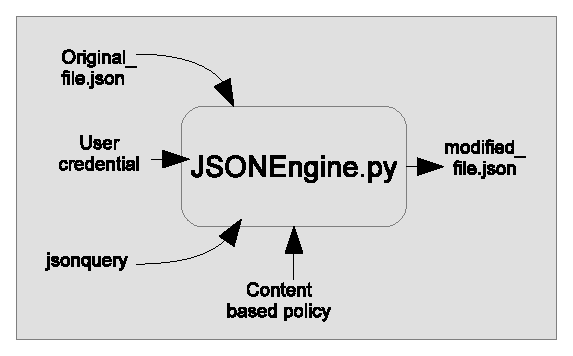
\includegraphics[width=0.3\textwidth]{eps/json_query_zap}
 \caption{The Skeleton for the CBAC zap.}
\label{fig:zappskeleton}
\end{figure}

\begin{enumerate}

  \item Attach a policy with a file/object stored in swift storage. The  file can be requested as it it, not it can be partially requested by specifying query parameter(jsonpath in our case) and instead of having the full content, the requester may get selective content based on his acting role. This case is explained in the above section. The skeleton for the to be developed zerovm application is shown in the figure \ref{fig:zappskeleton}





\item Attach a policy at the container label 

\end{enumerate}









